\documentclass{article}

\usepackage{fullpage}
\usepackage{array}
\usepackage{amsmath,amssymb,amsfonts,mathrsfs,amsthm}
\usepackage[utf8]{inputenc}
\usepackage{listings}
\usepackage{mathtools}
\usepackage{pdfpages}
\usepackage[textsize=footnotesize,color=green]{todonotes}
\usepackage{bm}
\usepackage{tikz}
\usepackage[normalem]{ulem}

\usepackage{graphicx}
\usepackage{subfigure}

\usepackage{color}
\usepackage{pdflscape}
\usepackage{pifont}

\usepackage{bibentry}
\nobibliography*

\renewcommand{\topfraction}{0.85}
\renewcommand{\textfraction}{0.1}
\renewcommand{\floatpagefraction}{0.75}

\newcommand{\vect}[1]{\ensuremath\boldsymbol{#1}}
\newcommand{\tensor}[1]{\underline{\vect{#1}}}
\newcommand{\del}{\triangle}
\newcommand{\grad}{\nabla}
\newcommand{\curl}{\grad \times}
\renewcommand{\div}{\grad \cdot}
\newcommand{\ip}[1]{\left\langle #1 \right\rangle}
\newcommand{\eip}[1]{a\left( #1 \right)}
\newcommand{\td}[2]{\frac{d#1}{d#2}}
\newcommand{\pd}[2]{\frac{\partial#1}{\partial#2}}
\newcommand{\pdd}[2]{\frac{\partial^2#1}{\partial#2^2}}

\newcommand{\circone}{\ding{192}}
\newcommand{\circtwo}{\ding{193}}
\newcommand{\circthree}{\ding{194}}
\newcommand{\circfour}{\ding{195}}
\newcommand{\circfive}{\ding{196}}

\newcommand{\Reyn}{\rm Re}

\newcommand{\bs}[1]{\boldsymbol{#1}}
\DeclareMathOperator{\diag}{diag}

\newcommand{\equaldef}{\stackrel{\mathrm{def}}{=}}

\newcommand{\tablab}[1]{\label{tab:#1}}
\newcommand{\tabref}[1]{Table~\ref{tab:#1}}

\newcommand{\theolab}[1]{\label{theo:#1}}
\newcommand{\theoref}[1]{\ref{theo:#1}}
\newcommand{\eqnlab}[1]{\label{eq:#1}}
\newcommand{\eqnref}[1]{\eqref{eq:#1}}
\newcommand{\seclab}[1]{\label{sec:#1}}
\newcommand{\secref}[1]{\ref{sec:#1}}
\newcommand{\lemlab}[1]{\label{lem:#1}}
\newcommand{\lemref}[1]{\ref{lem:#1}}

\newcommand{\mb}[1]{\mathbf{#1}}
\newcommand{\mbb}[1]{\mathbb{#1}}
\newcommand{\mc}[1]{\mathcal{#1}}
\newcommand{\nor}[1]{\left\| #1 \right\|}
\newcommand{\snor}[1]{\left| #1 \right|}
\newcommand{\LRp}[1]{\left( #1 \right)}
\newcommand{\LRs}[1]{\left[ #1 \right]}
\newcommand{\LRa}[1]{\left\langle #1 \right\rangle}
\newcommand{\LRb}[1]{\left| #1 \right|}
\newcommand{\LRc}[1]{\left\{ #1 \right\}}

\newcommand{\Grad} {\ensuremath{\nabla}}
\newcommand{\Div} {\ensuremath{\nabla\cdot}}
\newcommand{\Nel} {\ensuremath{{N^\text{el}}}}
\newcommand{\jump}[1] {\ensuremath{\LRs{\![#1]\!}}}
\newcommand{\uh}{\widehat{u}}
\newcommand{\fnh}{\widehat{f}_n}
\renewcommand{\L}{L^2\LRp{\Omega}}
\newcommand{\pO}{\partial\Omega}
\newcommand{\Gh}{\Gamma_h}
\newcommand{\Gm}{\Gamma_{-}}
\newcommand{\Gp}{\Gamma_{+}}
\newcommand{\Go}{\Gamma_0}
\newcommand{\Oh}{\Omega_h}

\newcommand{\eval}[2][\right]{\relax
  \ifx#1\right\relax \left.\fi#2#1\rvert}

\def\etal{{\it et al.~}}


\def\arr#1#2#3#4{\left[
\begin{array}{cc}
#1 & #2\\
#3 & #4\\
\end{array}
\right]}
\def\vecttwo#1#2{\left[
\begin{array}{c}
#1\\
#2\\
\end{array}
\right]}
\def\vectthree#1#2#3{\left[
\begin{array}{c}
#1\\
#2\\
#3\\
\end{array}
\right]}
\def\vectfour#1#2#3#4{\left[
\begin{array}{c}
#1\\
#2\\
#3\\
#4\\
\end{array}
\right]}

\newcommand{\G} {\Gamma}
\newcommand{\Gin} {\Gamma_{in}}
\newcommand{\Gout} {\Gamma_{out}}


\title{General notes on DPG}
\begin{document}
\maketitle

\section{Least squares}

We begin with a general variational formulation 
\[
b(u,v) = l(v)
\]

DPG begins with the idea that you would like to do least squares on the operator equation 
\[
Bu = \ell, \quad Bu, \ell \in V'
\]
where $\LRa{Bu,v}_{V'\times V} = b(u,v)$ and $\LRa{\ell, v}_{V'\times V} = l(v)$.  Since $Bu - \ell \in V'$, we minimize the norm of this residual in $V'$ over the finite dimensional space $U_h$, i.e. 
\[
\min_{u_h \in U_h} \nor{Bu_h - \ell}_{V'}^2.
\]
This leads to the normal equations 
\[
\LRp{Bu-\ell, B\delta u}_{V'}, \quad \forall \delta u \in U_h.
\]
The Riesz map gives us the equivalent definition 
\[
\LRp{R_V^{-1}\LRp{Bu-\ell}, R_V^{-1}\LRp{B\delta u}}_{V} = 0, \quad \forall \delta u \in U_h.
\]
Assuming we've specified the Riesz map through a test space inner product
\[
\LRa{R_V v , \delta v}_{V'\times V}= (v,\delta v)_V,
\]
this leads to what I call a Dual Petrov-Galerkin method.  

\section{Algebraic perspective} 

In the above example, $V$ is infinite dimensional.  If we approximate $V$ by $V_h$ such that $\dim (V_h) > \dim (U_h)$, we get matrix representations of our operators
\begin{align*}
B_{ij} &= b(u_j, v_i), \quad u_j \in U_h, v_i \in V_h\\
R_V &= (v_i,v_j)_V \quad  v_i,v_j\in V_h\\
\ell_i &= l(v_i), \quad v_i \in V_h.
\end{align*}
The resulting normal equations 
\[
\LRp{R_V^{-1}\LRp{Bu-\ell}, R_V^{-1}\LRp{B\delta u}}_{V}, \quad \forall \delta u \in U_h.
\]
can now be written as 
\[
\LRp{R_V^{-1}\LRp{Bu-\ell}}^T R_V \LRp{R_V^{-1}B} = 0, 
\]
or, after simplifying to $\LRp{Bu-\ell}^T R_V^{-1} B = 0$, we get the algebraic normal equations
\[
B^TR_V^{-1}Bu = B^TR_V^{-1} \ell.
\]
This is just the solution to the algebraic least squares problem
\[
\min_u \nor{Bu-\ell}_{R_V^{-1}}^2.
\]
Such problems can also be written using the augmented system for the least squares problem
\[
\arr{R_V}{B}{B^T}{0}\vecttwo{e}{u} = \vecttwo{l}{0}.
\]
This can be interpreted as the mixed form of the Dual Petrov-Galerkin method, which is used by Cohen, Welper, and Dahmen in their 2012 paper ``Adaptivity and variational stabilization for convection-diffusion equations''.  
\begin{align*}
(e,v)_V + b(u,v) &= l(v) \\
b(\delta u,e) &= 0
\end{align*}
Eliminating $e$ from the above system leads to the above algebraic normal equations.  

\emph{Note: for general $R_V$, the algebraic normal equations are completely dense.  Cohen, Welper, and Dahmen thus solve the augmented system to get solutions in this setting; however, this is a saddle point problem, and over 2x as large as the trial space, which makes preconditioning and solving more difficult. }

\section{Deriving the Discontinuous Petrov-Galerkin method}
We want to avoid solving either a fully dense system or a saddle point problem, so we introduce Lagrange multipliers $\uh$ to enforce continuity weakly on $e$, which we will now approximate using discontinuous functions.  These $\uh$ are defined on element edges only, similarly to hybrid variables or mortars in finite elements.  This leads to the new system 
\begin{align*}
\LRa{\uh, \jump{v}}_{\Gh} + (e,v)_V + b(u,v) &= l(v) \\
b(\delta u,e) &= 0\\
\LRa{\hat{\mu}, \jump{e}}_{\Gh} &= 0
\end{align*}
where $\Gh$ is the mesh skeleton (union of all element edges).  The resulting algebraic system here is 
\[
\left[
\begin{array}{c c c}
R_V & B& \hat{B}\\
B^T & 0& 0\\
\hat{B}^T & 0& 0
\end{array}
\right]
\left[\begin{array}{c}
e \\ u\\ \uh
\end{array}
\right]
= 
\left[\begin{array}{c}
f\\0\\0
\end{array}
\right].
\]
Because $e$ is now discontinuous, $R_V$ is made block-diagonal; eliminating $e$ returns the (fairly) sparse symmetric positive-definite DPG system
\[
A = \left[\begin{array}{c c}
B^TR_V^{-1}B & B^TR_V^{-1}\hat{B}\\
\hat{B}^TR_V^{-1}B & \hat{B}^TR_V^{-1}\hat{B}
\end{array}\right]
\vecttwo{u}{\uh} = \vecttwo{B^TR_V^{-1} f}{\hat{B}^TR_V^{-1}f}.
\]

\subsection{Primal hybrid formulation: why it works for DPG}

Note: primal hybrid formulation gives Crouziex-Raviart elements for lowest order $N=1$, with flux order $N_f = N-1$.  However, this does not work in defining elements for $N>1$; for $N$ even and $N_f = N-1$, the Lagrange multiplier constraint set will not be linearly independent.   On triangles, the jump constraints for $N$ odd will imply that the solution must be an orthogonal polynomial of order $N$ over the edge.  Since $N$ is odd, in 2D, the values at both vertices will be equal, and the trace on the edge will be continuous.  Taking $u$ to be any polynomial over $T$ with this trace gives that $Bu = 0$, but $u\neq 0$.  (I believe Jay Gopalakrishnan also noticed this independently.)

If you take $N$ arbitrary and $N_f \leq N-2$, however, things work fine.  This is roughly the situation with DPG - consider primal DPG, with $N_{\rm trial}$, $N_{\rm test} = N_{\rm trial} + 2$, and $N_f = N_{\rm trial} - 1$.  

%\section{Ideas from domain decomposition}
%
%The DPG method can be considered a 
%\begin{figure}
%\centering
%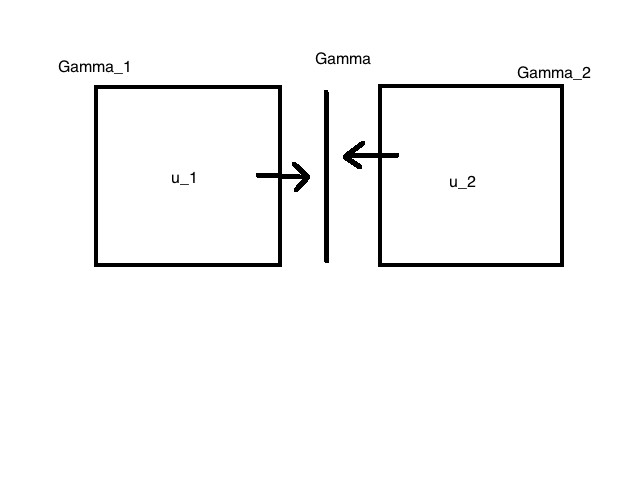
\includegraphics[width=.6\textwidth]{figs/DDdiagram.png}
%\end{figure}

\section{Primal DPG and preconditioning}

The DPG system can be reordered 
\[
A = \left[\begin{array}{c c}
B^TR_V^{-1}B & B^TR_V^{-1}\hat{B}\\
\hat{B}^TR_V^{-1}B & \hat{B}^TR_V^{-1}\hat{B}
\end{array}
\right] = \arr{K}{C}{C^T}{F}
\]
where $K$ is the matrix corresponding to field (volume) variables, $F$ is the submatrix corresponding to flux (surface/mortar) variables, and $C$ couples the system together.  

We can do a block triangular factorization of this system 
\[
A = \arr{I}{0}{C^TK^{-1}}{I}\arr{K}{0}{0}{S}\arr{I}{K^{-1}C}{0}{I}.
\]
where $S = F - C^TK^{-1}C$, the Schur complement.  We approach the design of preconditioners based on the approximate inversion of $K$ and $S$.  

For a first pass, we consider the primal DPG method, which is probably the simplest DPG method available, where field variables are approximated with $C_0$-continuous piecewise polynomials and the flux variables are approximated using discontinuous mortar basis functions.  Test functions are approximated with disjoint discontinuous polynomials of higher order than the trial field variables.  

We may also wish to consider the DPG method with ultra-weak variational formulation (discontinuous field variables).  In this case, $K$ is also block diagonal.  

\subsection{$K$ block}

We assume that preconditioning the $K$ submatrix can roughly be done using similar techniques to preconditioning standard elliptic equations.  Initial numerical evidence appears to support this

\begin{itemize}
\item Two-level additive Schwarz.  A coarse solve ($P_1$ elements with AGMG?) + (overlapping) block solves.  \textcolor{red}{Not working yet.}
\item Direct AGMG preconditioning.  \textcolor{red}{Working for CG and DPG.}
\item $P_1$ FEM preconditioning of nodal bases \textcolor{red}{Working for CG, not yet implemented for DPG.}
\end{itemize}

\subsection{Schur block}

Preconditioners for this general sort of system often involve an approximation of the Schur complement, which, in this case, is
\[
S = \hat{B}^TR_V^{-1}\hat{B} - \hat{B}^TR_V^{-1}{B}\LRp{B^TR_V^{-1}B}^{-1} B^TR_V^{-1}\hat{B}
\]
Factoring out $\hat{B}$ on both sides gives
\[
S = \hat{B}^T\LRp{R_V^{-1} - R_V^{-1}{B}\LRp{B^TR_V^{-1}B}^{-1} B^TR_V^{-1}}\hat{B}
\]
Factoring out $\hat{B}^TR_V^{-1}$ on both the left and right gives
\[
S = \hat{B}^TR_V^{-1}\LRp{R_V-B\LRp{B^TR_V^{-1}B}^{-1}B^T}R_V^{-1}\hat{B}
\]
If we define $\tilde{B} = R_V^{-1/2}{B}$, then the above is
\[
S = \hat{B}^TR_V^{-1/2}\LRs{I - \tilde{B}(\tilde{B}^T\tilde{B})^{-1}\tilde{B}^T}R_V^{-1/2}\hat{B}.
\]
The matrix $\LRs{I - \tilde{B}(\tilde{B}^T\tilde{B})^{-1}\tilde{B}^T}$ is the orthogonal projector onto the kernel of $\tilde{B}^T$ - does this help? 

Alternatively, suppose we just wish to precondition $S$ with $C = \hat{B}^TR_V^{-1}\hat{B}$.  This assumes that $C^{-1}S = I - C^{-1}B^TA^{-1}B$ is close to an identity, or that $C^{-1}B^TA^{-1}B$ is nearly zero.  Numerical experiments with Poisson/convection-diffusion indicate this may holds independently of $h$, though convection-diffusion appears to have dependence on $N$ for $N>4$.  

\subsection{Block Jacobi}

We can write (overloading notation for $A$) the full DPG system in block form
\[
\arr{A}{B}{B^T}{C}\vecttwo{u}{\uh} = \vecttwo{f}{g}.
\]
We could naively break the system up into two blocks and use a fixed point iterative scheme
\begin{align*}
u^{n+1} &= A^{-1}(f-B\uh^{n})\\
\uh^{n+1} &= C^{-1}(g-B^Tu^{n+1}).
\end{align*}
or equivalently
\[
\vecttwo{u}{\uh} = \arr{A^{-1}}{}{}{C^{-1}}\LRp{\vecttwo{f}{g} - \arr{}{B}{B^T}{}\vecttwo{u}{\uh}}
\]
which we can recognize as a block Jacobi iteration.  This may be preferrable in a matrix-free environment, as both $A$ and $C$ can be computed in a matrix-free fashion ($C\uh$ can be computed using local inversions of the Riesz product with $\uh$ as boundary data).  As far as I can tell, the Schur complement $S = C-B^TA^{-1}B$ for a general DPG system cannot.

This iteration was tested on pure convection under both the ultra-weak and primal formulations.  As there was no observable difference in the primal formulation, we just show ultra-weak results here.  
\begin{itemize}
\item Convergence depends on $\Delta N$ and $N_{\rm flux}$.  
\item If $N_{\rm flux} = 0$, convergence is roughly independent of $\Delta N$.  If $N_{\rm flux} > 0$, the convergence is both slower than with $N_{\rm flux} = 0$ and more sensitive to $N$ and $\Delta N$.
\end{itemize}

Convergence of the fixed point solution to the exact solution is shown here.
\begin{figure}
\centering
\subfigure[$N_{\rm flux} = 1, \Delta N = 2$]{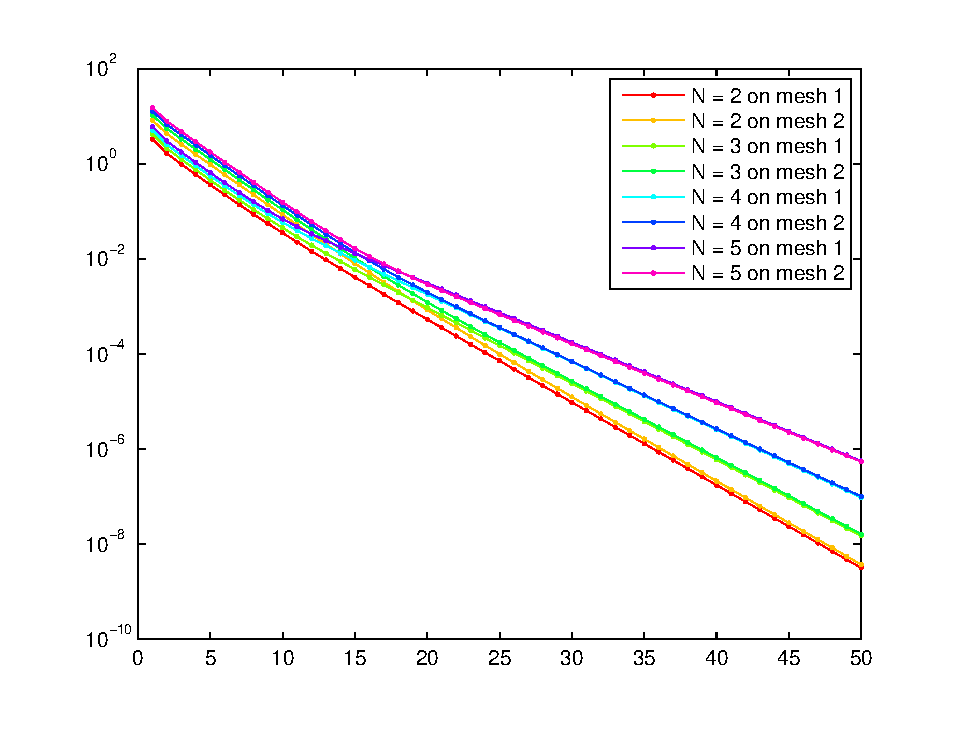
\includegraphics[width=.49\textwidth]{figs/Nflux1_DP2.eps}}
\subfigure[$N_{\rm flux} = 1, \Delta N = 4$]{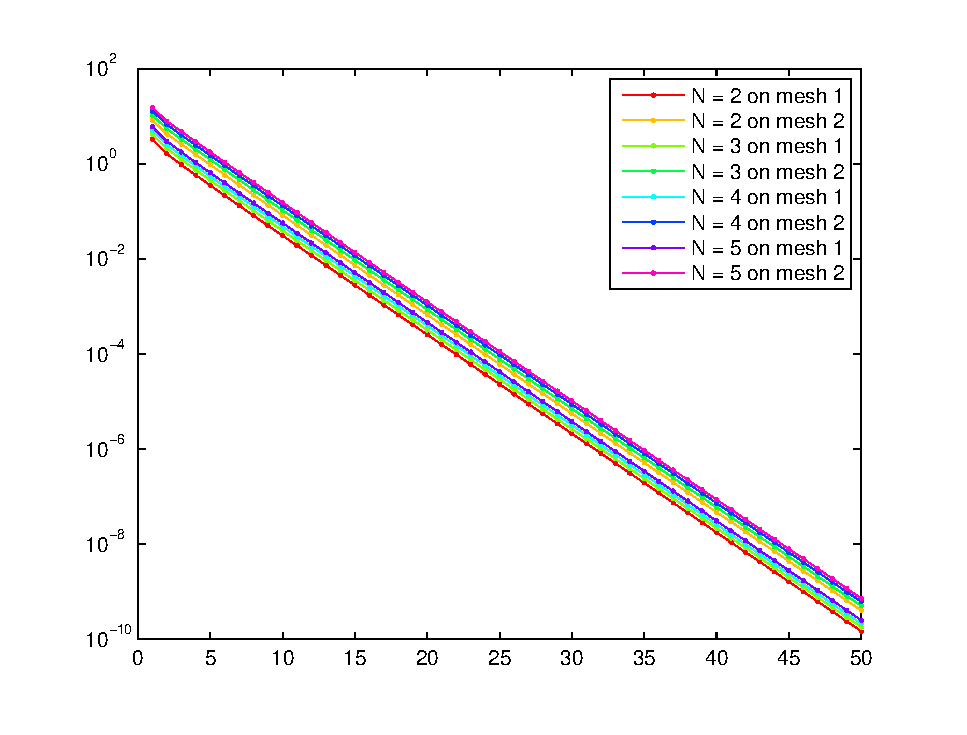
\includegraphics[width=.49\textwidth]{figs/Nflux1_DP4.eps}}
\subfigure[$N_{\rm flux} = 0, \Delta N = 4$]{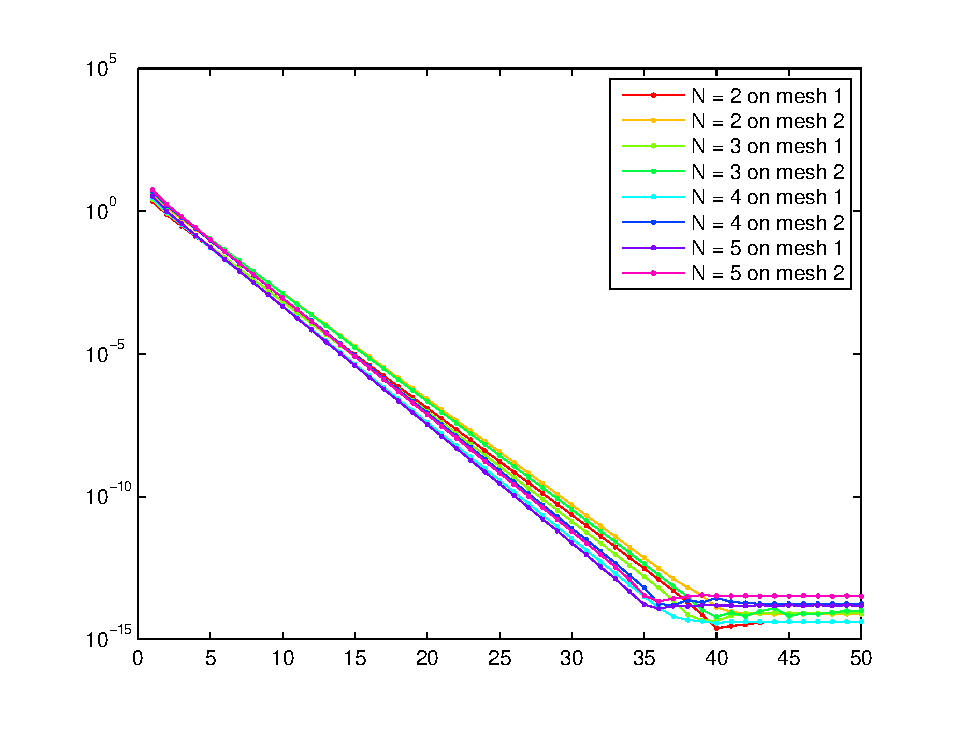
\includegraphics[width=.49\textwidth]{figs/Nflux0_DP2.eps}}
\subfigure[$N_{\rm flux} = 0, \Delta N = 2$]{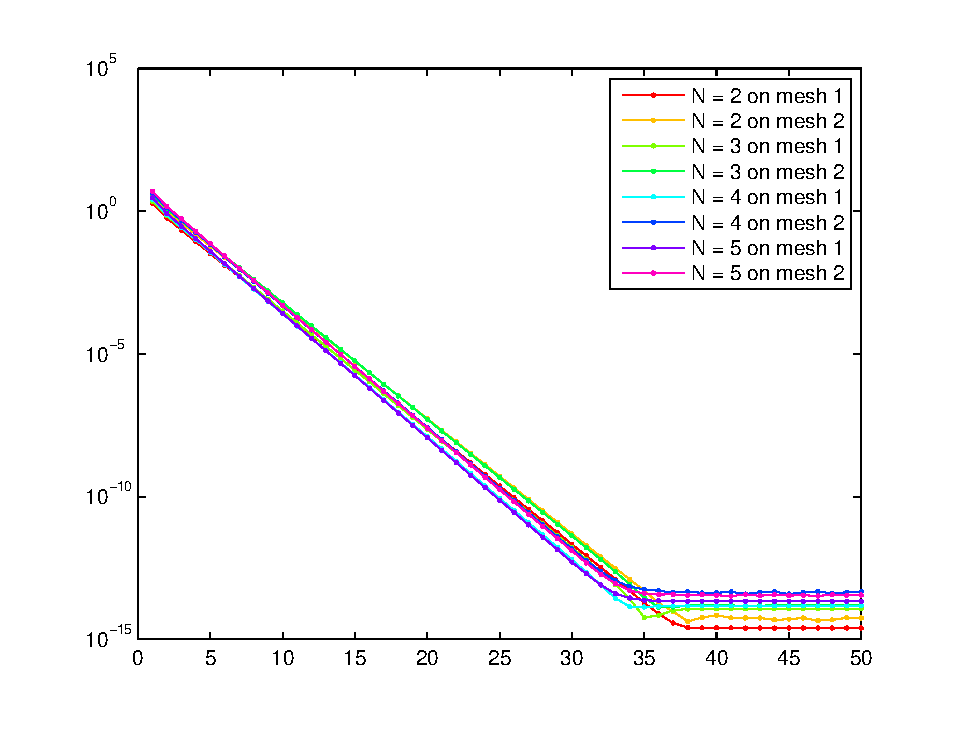
\includegraphics[width=.49\textwidth]{figs/Nflux0_DP4.eps}}
\caption{Block Jacobi fixed point iterations for pure convection with $\beta = (1,0)$, ultra-weak formulation.}
\end{figure}

Questions:
\begin{itemize}
\item Do the results carry over for the ultra-weak formulation?
\item Why do these results fail for Poisson's equation in the primal formulation?  
\item \textbf{This has to be related to the fixed point/Uzawa iteration of Dahmen.  How to prove?}
\end{itemize}

\subsection{Etc notes}
\begin{itemize}
\item Flux sub-block
\[
\hat{B}R_V^{-1}\hat{B}
\]
is the exact same as system for primal hybrid method under the test norm.  Block preconditioner?
\item Can we use the idea of reducing to field dofs?  i.e. turn the inversion of the flux matrix into just an outer product?  Make equiv to testing with null space of $\hat{B}^T$...
\item Can we change the coupling to the mortar space for $e$?  i.e. add consistency/penalty/etc?
\item Mesh dependent test norms: do they improve the flux subproblem?  
\item Calderon preconditioners?
\end{itemize}

\end{document}

